\section{Results and Tests}

Measurements were done for both the polling based system \ref{subsection:polling} and the low energy mode based system \ref{subsection:low-energy}. A repeat pattern of button presses were executed in each mode, and measured.

\subsection{Polling based system}

As can be seen in the figure \ref{fig:polling-based-system}, the system uses a significant amount of power.
There is a slight spike when buttons are pressed, but the increased amount of power draw is negligible compared to the average draw.

The power usage when the program is running averages about 4 $m A$

\begin{figure}[h]
\centering
\includegraphics[width=\textwidth]{figures/polling.pdf}
\caption{Polling based system}
\label{fig:polling-based-system}
\end{figure}

\subsection{Low energy mode based system}
In figure \ref{fig:sleep-based-system}, the difference between the times the processor is sleeping, and when buttons are pressed can easily be seen.
Some variance in the measurements are visible, these are due transients as the voltage settles to its new value.

The power usage when the program is sleeping averages about 1.8 $\mu A$.

\begin{figure}[h]
\centering
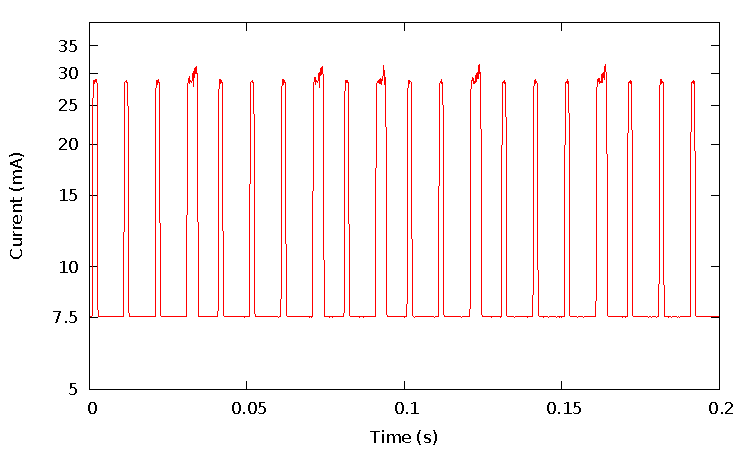
\includegraphics[width=\textwidth]{figures/sleep.pdf}
\caption{Sleep based system}
\label{fig:sleep-based-system}
\end{figure}

\subsection{System comparison}

The system comparison clearly shows the payoff of using a low energy mode when idling.



\begin{figure}[h]
\centering
\includegraphics[width=\textwidth]{figures/all.pdf}
\caption{System comparison}
\label{fig:system-comparison}
\end{figure}
